%% ----------------------------------------------------------------
%% PACKAGES
%% ----------------------------------------------------------------
\documentclass[titlepage, 12pt]{article}
\usepackage[dvipsnames]{xcolor}     %first needed because tikz
\usepackage[utf8]{inputenc}
\usepackage[spanish]{babel}
\usepackage{amsmath}
\usepackage{biblatex}
\usepackage{booktabs}
\usepackage[RPvoltages]{circuitikz}
\usepackage{csquotes}   %used by biblatex
\usepackage{enumitem}
\usepackage{fancyhdr}
\usepackage{float}
\usepackage{geometry} 
\usepackage{graphicx}
\usepackage[hidelinks]{hyperref}
\usepackage{pdflscape}
\usepackage{parskip}
\usepackage{siunitx}
\usepackage{subcaption}
\usepackage{tikz}
\usepackage{xfrac}
\usepackage[dvipsnames]{xcolor}

% Custom package for non italic uppercase
% inside equations
%%\usepackage{nonitalic_upper}

%% ----------------------------------------------------------------
%% PACKAGE SETTINGS
%% ----------------------------------------------------------------
\decimalpoint
\geometry{
 a4paper,
 total={170mm,247mm},   %210x297mm
 left=20mm,
 top=20mm,
}
%\setlength\headheight{30pt}

%% ----------------------------------------------------------------
%% TITLE
%% ----------------------------------------------------------------
\title{Plan de proyecto:\\Calibrador y caracterizador de sondas de corriente}
\author{Agustín Aon Sanchez\\ 
Facultad de Ingeniería\\
Universidad Nacional de Mar del Plata}
\date{Seminario de proyecto final\\Revisión 1}

%% ----------------------------------------------------------------
%% BEGIN
%% ----------------------------------------------------------------
\begin{document}
\maketitle

\renewcommand{\tablename}{Tabla}
%% ----------------------------------------------------------------
%% DOCUMENT
%% ----------------------------------------------------------------

%% ----------------------------------------------------------------
\section*{Plan de proyecto}
%% ----------------------------------------------------------------
El proyecto final comenzó en diciembre de 2019. Se planteó en ese primer comienzo el diagrama en bloques del sistema a desarrollar y se comenzó con una investigación de sensores de corriente, técnicas de generación de corriente y aprendizaje de C y Python. Este proceso llevó aproximadamente 1 mes.

A lo largo del año 2020 y principios de 2021 se realizó lo que se describe a continuación.

Se diseñó primero el firmware que correría el microcontrolador. El desarrollo del mismo llevó aproximadamente 3 meses hasta obtener una primera iteración. El objetivo planteado fue obtener un firmware funcional, con una capa de comunicaciones y con una etapa de procesamiento de muestras.

Se diseñó luego el sistema de control. Para ello se realizó un estudio preliminar de los diferentes métodos de control de señales alternas, a través de publicaciones y libros especializados. Luego se procedió a realizar simulaciones para comprobar el funcionamiento. Este proceso llevó aproximadamente 1 mes.

Se continuó luego con el diseño del software, es decir la interfaz del programa en la PC. Se analizaron primero las diferentes alternativas de librerías, hasta que se eligió una y se procedió en el diseño. Este proceso llevó aproximadamente 3 meses.

Se realizó finalmente el diseño del hardware. Para ello se analizó primero versiones existentes de otros instrumentos desarrollados por el Laboratorio, se diseñaron luego los distintos módulos y finalmente se diseñó el PCB. 

En lo que resta del año 2021, se espera poder continuar con las tareas nombradas en la \autoref{tab:tareas} de acuerdo al esquema planteado en el diagrama de Gantt de la \autoref{fig:gantt}.
 
Se plantea completar la documentación necesaria para realizar la inscripción del proyecto final, para luego de concluída concurrir al Laboratorio y comenzar el montado de componentes en el PCB. Asimismo, se divide este proceso en dos etapas: soldado y prueba de módulos funcionales. En paralelo a estas tareas se espera completar el desarrollo de firmware y software, para que una vez terminado se pueda realizar la prueba final.


\begin{landscape}
    \thispagestyle{empty}

    \null\vfill

    \begin{table}[!hbtp]
        \centering
        \begin{tabular}{@{}lcc@{}}
            \toprule
            \multicolumn{1}{c}{Tarea} & \multicolumn{1}{c}{Fecha de inicio} & \multicolumn{1}{c}{Fecha de finalización} \\ \midrule
            Inscripción proyecto      & 12/04/21                            & 16/04/21                                  \\
            Soldar componentes en PCB & 19/04/21                            & 30/04/21                                  \\
            $\rightarrow$ Soldado por etapas        & 19/04/21                            & 23/04/21                                  \\
            $\rightarrow$ Prueba general            & 26/04/21                            & 30/04/21                                  \\
            Desarrollo firmware       & 12/04/21                            & 04/06/21                                  \\
            Desarrollo software       & 12/04/21                            & 04/06/21                                  \\
            Prueba final              & 07/06/21                            & 18/06/21                                  \\ \bottomrule
        \end{tabular}
        \caption{Lista de tareas}
        \label{tab:tareas}
    \end{table}
    
    \begin{figure}[!hbtp]
        \centering
        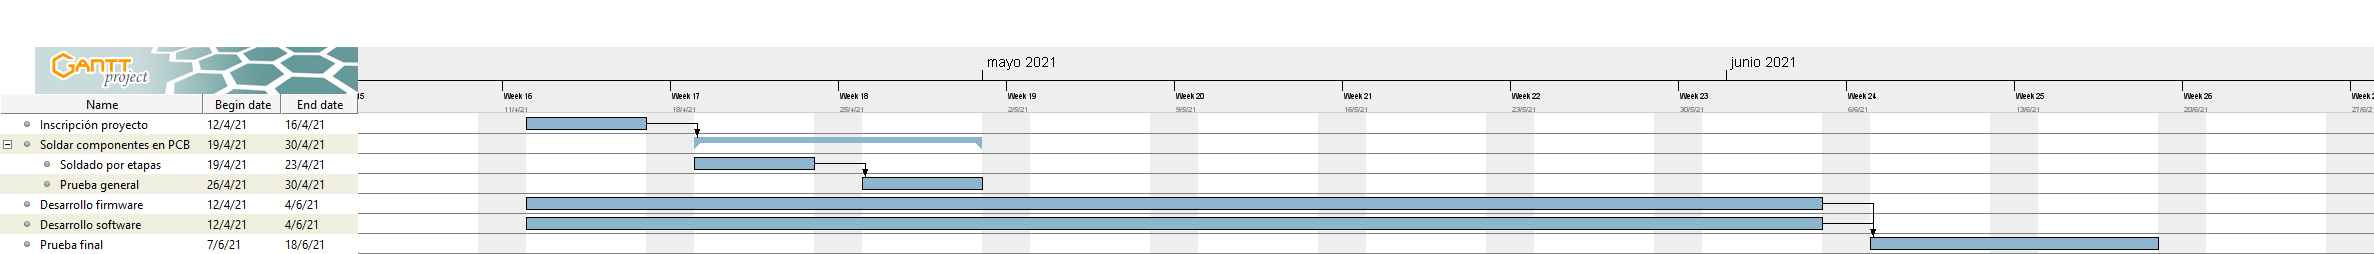
\includegraphics[scale=0.3]{proyecto.png}
        \caption{Esquema de tareas}
        \label{fig:gantt}
    \end{figure}
    
    \vfill\null
    \raisebox{-0em}{\makebox[\linewidth]{\thepage}}

\end{landscape}

\end{document}

